\documentclass[conference]{conference-latex-template_10-17-19/IEEEtran}
\IEEEoverridecommandlockouts

\usepackage{cite}
\usepackage{amsmath,amssymb,amsfonts}
\usepackage{graphicx}
\usepackage{textcomp}
\usepackage{xcolor}
\usepackage{booktabs}
\usepackage{adjustbox}
\usepackage{tikz}
\usetikzlibrary{arrows.meta,positioning,fit,calc,shapes.geometric}

\setlength{\textfloatsep}{7pt plus 1pt minus 1pt}
\setlength{\floatsep}{7pt plus 1pt minus 1pt}
\setlength{\intextsep}{7pt plus 1pt minus 1pt}
\setlength{\abovecaptionskip}{3pt}
\setlength{\belowcaptionskip}{2pt}
\renewcommand{\arraystretch}{0.94}

\def\BibTeX{{\rm B\kern-.05em{\sc i\kern-.025em b}\kern-.08em
    T\kern-.1667em\lower.7ex\hbox{E}\kern-.125emX}}

\begin{document}

\title{PulseFormer: Structure-Controllable Multi-Track Electronic Music Generation for DAW Workflows}

\author{
\IEEEauthorblockN{Zhenyu Xiong}
\IEEEauthorblockA{\textit{Shanghai Film Academy}\\
\textit{Shanghai University}\\
Shanghai, China\\
yaralastudio@shu.edu.cn}
\and
\IEEEauthorblockN{Yonghua Zhu*}
\IEEEauthorblockA{\textit{Shanghai Film Academy}\\
\textit{Shanghai University}\\
Shanghai, China\\
zyh@shu.edu.cn\\
*Corresponding author}
}

\maketitle

\begin{abstract}
This paper presents PulseFormer, a hybrid symbolic music-processing pipeline for structure-controllable multi-track Electronic Music generation. The system targets Digital Audio Workstation (DAW) workflows where generated material must remain editable as stems, structurally transparent, and renderable for listening evaluation. PulseFormer combines three design choices: a Time-Major compound-token representation that keeps concurrent cross-track events local in the sequence, a structural-density condition injected through both a prefix token and Feature-wise Linear Modulation (FiLM), and Temporal Anchor Stitching for long-form arrangement generation. Time-Major serialization reduces the average token distance between simultaneous cross-track events from thousands of tokens to 5.2. FiLM improves local 8-bar density response from weak correlation to near-perfect local density response ($r=0.997$), while a deterministic section scheduler and stitching procedure extend generation to 128-bar arrangements. Objective and perceptual evaluations indicate improved structural controllability and qualified-note rate over trained symbolic baselines, while groove-pattern similarity remains below a Track-Major baseline. The contribution is therefore positioned as a transparent, production-oriented music-processing framework rather than a claim of general musical-quality superiority.
\end{abstract}

\begin{IEEEkeywords}
symbolic music generation, multi-track composition, Transformer, structural control, FiLM, electronic music, DAW workflow
\end{IEEEkeywords}

\section{Introduction}
Symbolic music generation remains important for production workflows because MIDI sequences can be edited, quantized, re-orchestrated, and rendered as separated stems \cite{huang2019music,dong2020muspy}. Modern audio-domain systems can generate realistic waveforms \cite{copet2023simple,agostinelli2023musiclm}, but they usually provide limited access to track-level structure and are difficult to revise inside a DAW. For Electronic Music, these practical requirements are especially strong: producers frequently manipulate section labels, track activation, density ramps, and stem-level mix decisions.

Existing symbolic Transformer models \cite{vaswani2017attention,hsiao2021compound,ens2020mmm} face two recurring difficulties in dense multi-track Electronic Music. First, Track-Major serialization places all events of one instrument before the next instrument, so concurrent events such as kick and bass downbeats can be separated by thousands of tokens. Second, most autoregressive models lack a simple mechanism for enforcing section-level density progression, for example the sparse-to-dense movement from Intro to Buildup and Drop. These issues are not only musical; they affect the engineering usability of generated material in downstream production.

PulseFormer addresses these limitations with a hybrid design. The model handles local event generation, while transparent production rules handle macro-structural constraints. The main contributions are: (1) a Time-Major compound-token representation that makes concurrent multi-track events locally visible to attention; (2) a dual-pathway structural-density control signal, using both a prefix token and FiLM; (3) Temporal Anchor Stitching for assembling long-form arrangements from local generations; and (4) a DAW-oriented evaluation protocol combining symbolic metrics and rendered-audio MOS tests.

\begin{figure*}[t]
\centering
\resizebox{0.92\textwidth}{!}{%
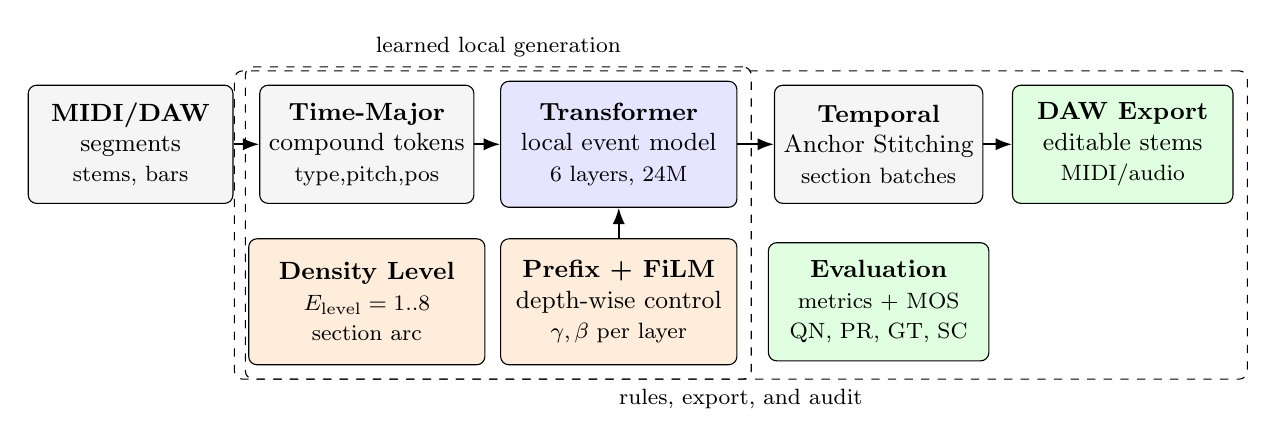
\begin{tikzpicture}[font=\small, >=Latex,
  stage/.style={draw, rounded corners=3pt, align=center, minimum width=26mm, minimum height=15mm, fill=gray!8},
  model/.style={draw, rounded corners=3pt, align=center, minimum width=30mm, minimum height=16mm, fill=blue!10},
  control/.style={draw, rounded corners=3pt, align=center, minimum width=30mm, minimum height=16mm, fill=orange!14},
  output/.style={draw, rounded corners=3pt, align=center, minimum width=28mm, minimum height=15mm, fill=green!12},
  line/.style={->, line width=0.65pt}]

\node[stage] (data) at (0,0) {\textbf{MIDI/DAW}\\segments\\{\footnotesize stems, bars}};
\node[stage] (token) at (3.0,0) {\textbf{Time-Major}\\compound tokens\\{\footnotesize type,pitch,pos}};
\node[model] (model) at (6.2,0) {\textbf{Transformer}\\local event model\\{\footnotesize 6 layers, 24M}};
\node[stage] (stitch) at (9.5,0) {\textbf{Temporal}\\Anchor Stitching\\{\footnotesize section batches}};
\node[output] (daw) at (12.6,0) {\textbf{DAW Export}\\editable stems\\{\footnotesize MIDI/audio}};

\node[control] (density) at (3.0,-2.0) {\textbf{Density Level}\\{\footnotesize $E_{\mathrm{level}}=1..8$}\\{\footnotesize section arc}};
\node[control] (film) at (6.2,-2.0) {\textbf{Prefix + FiLM}\\depth-wise control\\{\footnotesize $\gamma,\beta$ per layer}};
\node[output] (eval) at (9.5,-2.0) {\textbf{Evaluation}\\{\footnotesize metrics + MOS}\\{\footnotesize QN, PR, GT, SC}};

\draw[line] (data) -- (token);
\draw[line] (token) -- (model);
\draw[line] (model) -- (stitch);
\draw[line] (stitch) -- (daw);
\draw[line] (film) -- (model);

\node[draw, dashed, rounded corners=3pt, fit=(token)(model)(film), inner sep=5pt,
      label={[font=\footnotesize]above:learned local generation}] {};
\node[draw, dashed, rounded corners=3pt, fit=(density)(stitch)(daw)(eval), inner sep=5pt,
      label={[font=\footnotesize]below:rules, export, and audit}] {};
\end{tikzpicture}}
\caption{PulseFormer workflow. The diagram highlights the main technical content: Time-Major tokenization reduces cross-track token distance; density control enters through both prefix tokens and FiLM; Temporal Anchor Stitching extends generation to full arrangements; DAW export and rendered-audio evaluation close the production loop.}
\label{fig:pipeline}
\end{figure*}

\section{Related Work}
Symbolic music generation has developed from piano-roll and adversarial multi-track systems to sequence models using event or compound-token representations \cite{dong2018musegan,huang2020remi,hsiao2021compound,zeng2021musicbert}. Track-Major systems such as MMM expose long-range conditional control, but their serialized track blocks can separate simultaneous musical events by large token distances \cite{ens2020mmm}. Descriptor-conditioned symbolic models demonstrate that high-level musical attributes can guide generation, yet they do not directly target stem-level DAW production or explicit Electronic Music density arcs \cite{wu2023musemorphose}. Recent controllable accompaniment work such as BandControlNet uses fine spatiotemporal controls, while audio-domain systems such as MusicGen and MusicLM focus on waveform generation rather than editable symbolic stems \cite{luo2024bandcontrolnet,copet2023simple,agostinelli2023musiclm}.

PulseFormer is positioned between these families. It keeps symbolic editability, uses a Transformer local event model, and delegates macro-structural enforcement to transparent production rules. This separation is important for conference-style engineering evaluation: the method can be audited at the representation, model, scheduler, rendering, and perceptual-evaluation stages rather than being evaluated only as a black-box generator.

\section{Method}
\subsection{Time-Major Compound Tokens}
Each musical event is represented as a five-field compound token:
\begin{equation}
\begin{split}
E(x_i)&=\sum_{F\in\mathcal{F}} W_F(\mathrm{id}_F(x_i)),\\
\mathcal{F}&=\{T,P,Pos,Dur,Vel\}.
\end{split}
\end{equation}
The position field encodes a 16th-note step within the bar. In contrast to Track-Major serialization, PulseFormer orders events primarily by musical time and secondarily by track. Kick, bass, chord, and melody events at the same step therefore occupy adjacent positions in the autoregressive sequence. This reduces the representational burden for local cross-track coordination, although it also increases token density and limits the raw model context to about 8 bars.

\begin{table}[t]
\caption{Compound-token vocabulary used by PulseFormer}
\label{tab:vocab}
\centering\small
\adjustbox{max width=\columnwidth}{
\begin{tabular}{@{}llr@{}}
\toprule
Field & Examples & Size \\ \midrule
Type & bass, chord, melody, drums, global & 10 \\
Pitch / attribute & notes, drums, section tags, key, BPM & 234 \\
Position & 16th-note steps plus special tokens & 20 \\
Duration & 1, 2, 4, 8, 16 steps plus special tokens & 10 \\
Velocity & four MIDI bins plus special tokens & 8 \\ \bottomrule
\end{tabular}}
\end{table}

\subsection{Structural Density Conditioning}
The density level $\mathbf{E}_{\mathrm{level}}$ is an ordinal control variable aligned with DAW production practice: low values correspond to sparse sections, middle values to buildups, and high values to drops. PulseFormer uses a dual pathway. A prefix token anchors the target section in early attention layers, while FiLM re-injects the same condition at every Transformer layer:
\begin{equation}
\tilde{h}_{\ell}=
\gamma_{\ell}(\mathbf{E}_{\mathrm{level}})\odot h_{\ell}+
\beta_{\ell}(\mathbf{E}_{\mathrm{level}}).
\end{equation}
Here $h_{\ell}$ is the hidden sequence at layer $\ell$, and $\gamma_{\ell},\beta_{\ell}$ are produced by a small MLP from the density embedding. The model uses 6 decoder-only Transformer layers, 8 attention heads, hidden size 512, SwiGLU feed-forward blocks, FlashAttention-compatible causal masking, and approximately 24.0M parameters including FiLM \cite{dao2022flashattention}.

\subsection{Density Score and Section Schedule}
For each bar $t$, PulseFormer maps production features $\phi_t$ to a structural score
\begin{equation}
D_t=\sum_{j=1}^{6}w_j\phi_{t,j},
\end{equation}
where the features summarize active stems, drum activity, bass activity, chord support, melody presence, and local onset density. The score is quantized into eight density levels. A sparse Intro maps to a low level, a Buildup maps to a middle level, and a Drop maps to a high level. The scheduler supplies this density arc explicitly, so long-form monotonicity is treated as hybrid model-plus-rule behavior rather than a fully learned planning ability.

\subsection{Section Generation and DAW Export}
Because Time-Major interleaving places many simultaneous events in a short local region, a single context window covers only a phrase. PulseFormer therefore generates sections separately according to a fixed DAW-like schedule. Each new section receives the final bars of the previous section as an anchor prefix, preserving grid alignment at boundaries. A lightweight post-processing stage applies density masks, diatonic penalties, track-activation checks, and stem export. This design makes the pipeline easier to inspect than a purely prompt-driven generator: section control, model response, symbolic validity, and rendered-audio quality can be diagnosed separately.

\subsection{Implementation and Reproducibility Notes}
The complete pipeline is implemented as a staged symbolic-to-rendered workflow. First, MIDI and DAW-derived segments are normalized to a common tempo grid and converted into Time-Major compound events. Second, each target section is assigned a structural label and an ordinal density level. Third, the Transformer samples local events under the prefix and FiLM condition. Finally, the generated section is checked by rule-based masks before being exported as editable stems. This order is intentionally conservative: invalid or degenerate material can be detected before audio rendering, while rendered stimuli remain traceable to their symbolic source.

The model-side configuration is kept compact for conference evaluation. All trained systems share the same tokenizer grid, hidden size, and causal decoding setting, so the main comparisons isolate representation topology and density conditioning rather than confounding architecture scale. The reported long-form controllability should therefore be interpreted as a system-level property: FiLM improves local response, while the scheduler and stitching procedure enforce macro-level section progression. This distinction is important because a high 128-bar monotonicity score alone would otherwise overstate the amount of long-range planning learned by the Transformer.

\section{Experiments}
\subsection{Setup}
All trained models use the same Electronic Music corpus, tokenizer grid, and rendering protocol. The corpus is built from externally obtainable MIDI sources, including GigaMIDI and Lakh-derived Electronic Music subsets, plus a small proprietary DAW-project portion used only for training-domain coverage \cite{fradet2024gigamidi,raffel2016lakh}. Baselines include a Track-Major MMM Transformer and a Time-Major CP Transformer without FiLM. Objective evaluation uses 8 prompts with 8 restarts per system, producing 64 generated arrangements for each trained condition. Perceptual evaluation uses 25 listeners, 8 prompts, and four 5-point Likert dimensions: Groove Tightness (GT), Structural Coherence (SC), Melodic Variety (MV), and Mix Clarity (MC). Audio stimuli are rendered with the same DAW template and normalized before listening tests.

For the listening study, all systems are evaluated under matched prompts. Participants hear rendered audio rather than raw MIDI because Electronic Music production quality depends on drum articulation, stem balance, and transition clarity. However, symbolic outputs are retained for inspection so that perceptual results can be connected back to objective failures such as missing stems, out-of-range notes, or section-density mismatch. This dual protocol reduces the risk of judging the model only by a single aggregate score.

\subsection{Representation Topology}
Table~\ref{tab:topology} summarizes the token-distance advantage of Time-Major ordering. The result does not by itself prove learned coordination; rather, it shows that PulseFormer exposes concurrent musical events to the model within a much shorter attention path. This topology is the main reason the system is appropriate for dense kick-bass-chord-melody synchronization.

\begin{table}[t]
\caption{Token distance for concurrent cross-track events}
\label{tab:topology}
\centering\small
\begin{tabular}{@{}lcc@{}}
\toprule
Encoding & Mean distance & Max distance \\ \midrule
Track-Major & $3{,}249\pm422$ & $6{,}155$ \\
\textbf{Time-Major} & $\mathbf{5.2\pm1.8}$ & $\mathbf{12}$ \\ \bottomrule
\end{tabular}
\end{table}

\subsection{Objective Results}
PulseFormer achieves the highest qualified-note rate among trained systems and complete monotonic section adherence under the scheduler (Table~\ref{tab:objective}). Beat-level alignment is identical across trained models because all use the same 16th-note quantized tokenizer. Groove Pattern Similarity is lower than the Track-Major baseline, which likely reflects context-adaptive drum variation under Time-Major ordering rather than a simple rhythmic failure. Qualified-note rate (QN\%) measures the proportion of notes surviving range, duration, and track-role checks; PCHE summarizes pitch-class entropy; and monotonicity checks whether section density follows the requested production arc.

\begin{table*}[t]
\caption{Objective comparison, mean$\pm$SD. BAS is non-discriminative due to the shared quantized grid}
\label{tab:objective}
\centering\small
\begin{tabular}{@{}lccccc@{}}
\toprule
System & GPS$\uparrow$ & BAS$\uparrow$ & QN\%$\uparrow$ & PCHE$\uparrow$ & Monotonicity$\uparrow$ \\ \midrule
MMM Transformer & $\mathbf{0.871\pm0.138}$ & 1.000 & $36.8\pm19.6$ & $\mathbf{2.19\pm0.39}$ & 33\% \\
CP Transformer & $0.768\pm0.162$ & 1.000 & $34.8\pm21.1$ & $2.28\pm0.36$ & 33\% \\
\textbf{PulseFormer} & $0.717\pm0.203$ & \textbf{1.000} & $\mathbf{42.5\pm29.6}$ & $2.17\pm0.51$ & \textbf{100\%} \\ \bottomrule
\end{tabular}
\end{table*}

\subsection{Ablation and Perceptual Results}
The ablation results separate local model behavior from pipeline-level control. Time-Major encoding removes one source of cross-track counting drift under the quantized evaluation protocol, but by itself has poor density response ($r=0.155$). Adding a density prefix raises local response to $r=0.781$, and FiLM raises it to $r=0.997$. With section stitching and the deterministic scheduler, 128-bar target adherence is $r=0.982$; this should be read as hybrid model-plus-rule behavior.

\begin{table}[t]
\caption{Additive ablation of core modules}
\label{tab:ablation}
\centering\small
\adjustbox{max width=\columnwidth}{
\begin{tabular}{@{}lcccc@{}}
\toprule
Variant & $\Delta_{sync}$ & GC & PR & ISR \\ \midrule
Track-Major & 915 ms & 29.1 & 0.600 & 53.2 \\
+ Time-Major & 0.0 ms & 61.8 & 0.155 & 54.2 \\
+ Prefix & 0.0 ms & 62.1 & 0.781 & 54.9 \\
+ FiLM & 0.0 ms & 62.5 & \textbf{0.997} & 55.3 \\
+ Harmonic & 0.0 ms & 62.1 & 0.992 & \textbf{73.1} \\
\textbf{+ Stitching} & 0.0 ms & \textbf{71.3} & 0.982 & 73.1 \\ \bottomrule
\end{tabular}}
\end{table}

Fig.~\ref{fig:ablation_heatmap} visualizes the same additive trend as a compact heatmap. The strongest discontinuity occurs when the density prefix and FiLM are added: the model no longer treats section labels as weak metadata but receives the control signal at every layer. The later harmonic penalty changes ISR more than structural response, showing that pitch validity and section density are partly separable objectives. Finally, stitching changes the operating regime from short local phrases to 128-bar arrangements, so its high PR score is interpreted as combined model-and-rule adherence.

\begin{figure}[t]
\centering
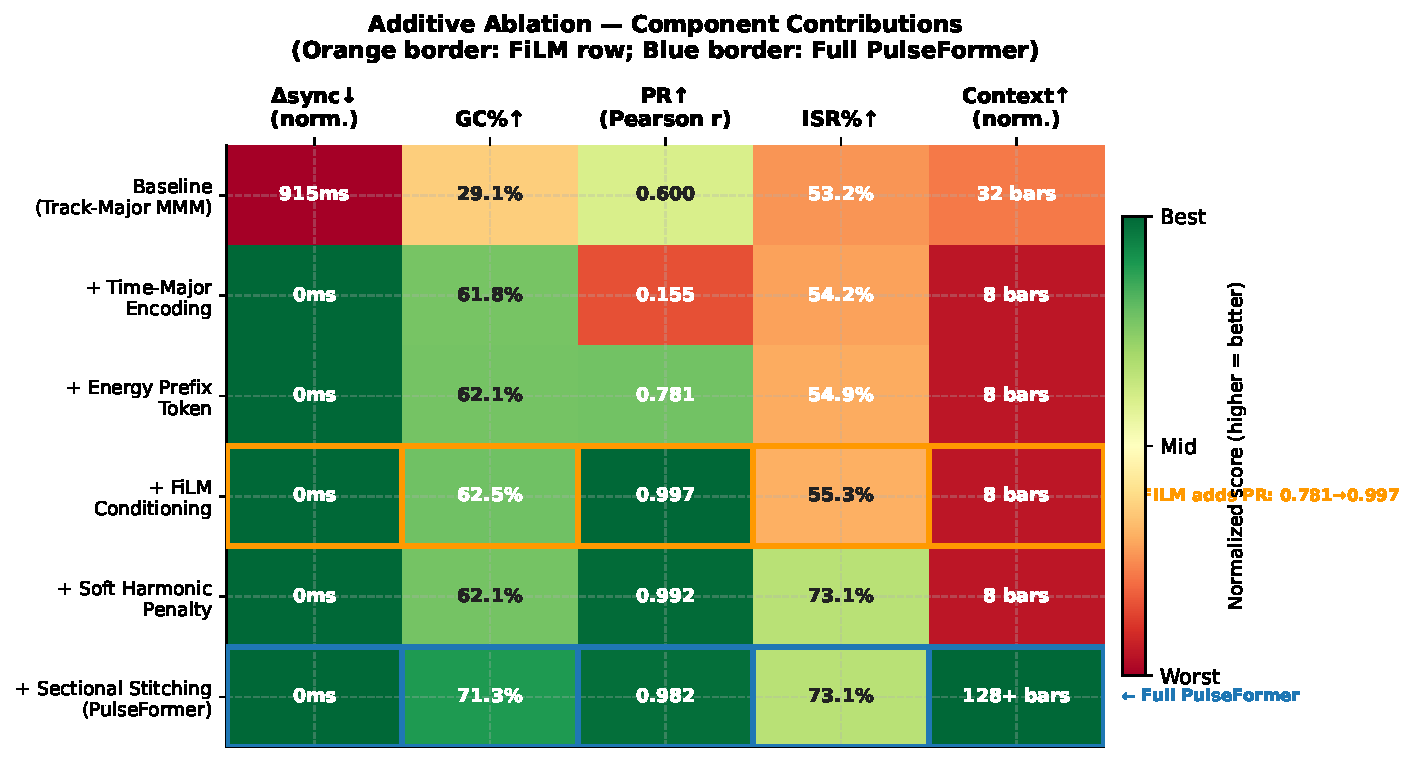
\includegraphics[width=\columnwidth]{figures/ablation_heatmap.pdf}
\caption{Ablation heatmap for PulseFormer modules. The visualization highlights the separation between local density conditioning, harmonic filtering, and long-form stitching.}
\label{fig:ablation_heatmap}
\end{figure}

The MOS study supports the same interpretation. PulseFormer is close to the human anchor on GT in this stimulus set and outperforms the baselines on SC and MC, while MV remains below the human reference. Because inter-rater agreement is only fair-to-moderate, the listening study is treated as supportive evidence rather than a distribution-level benchmark.

The main qualitative observation from the MOS profile is that PulseFormer improves the production-facing dimensions most directly targeted by the pipeline. GT benefits from strict grid preservation, and SC benefits from explicit section-density control. MV remains weaker because the same constraints that stabilize dense drops also limit unconstrained melodic wandering. This trade-off is acceptable for the target use case, where the system is intended to provide editable structural material for producers rather than final human-level compositions.

\begin{table}[t]
\caption{MOS results, 8 prompts $\times$ 25 listeners}
\label{tab:mos}
\centering\small
\adjustbox{max width=\columnwidth}{
\begin{tabular}{@{}lcccc@{}}
\toprule
System & GT & SC & MV & MC \\ \midrule
Human & $3.91\pm0.52$ & $\mathbf{4.24\pm0.54}$ & $\mathbf{4.06\pm0.47}$ & $\mathbf{3.90\pm0.59}$ \\
\textbf{PulseFormer} & $\mathbf{3.98\pm0.57}$ & $3.76\pm0.64$ & $2.92\pm0.63$ & $3.52\pm0.61$ \\
CP Transformer & $3.64\pm0.58$ & $2.70\pm0.64$ & $2.82\pm0.61$ & $3.10\pm0.64$ \\
MMM Transformer & $3.06\pm0.62$ & $2.14\pm0.62$ & $2.48\pm0.63$ & $2.34\pm0.70$ \\ \bottomrule
\end{tabular}}
\end{table}

\begin{figure}[t]
\centering
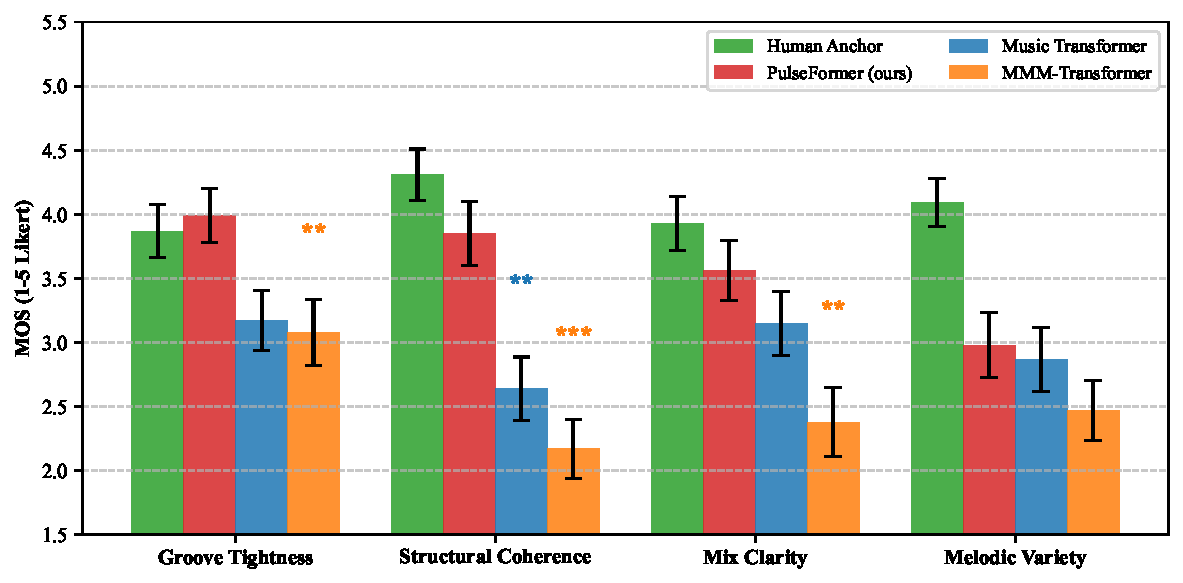
\includegraphics[width=0.84\columnwidth]{figures/radar.pdf}
\caption{Rendered-audio MOS profile. PulseFormer is strongest on grid tightness and structural coherence, while melodic variety remains below the human anchor.}
\label{fig:mos}
\end{figure}

\section{Discussion and Conclusion}
PulseFormer demonstrates that controllable symbolic generation for Electronic Music benefits from combining model design with transparent production rules. Time-Major topology makes concurrent multi-track events local in the sequence. FiLM makes the density condition persistent across Transformer depth. Temporal Anchor Stitching enables long-form output while retaining editable DAW stems. These design choices directly serve conference-style engineering criteria: a clearly defined problem, a reproducible pipeline, compact measurable improvements, and explicit limitations.

In a practical production scenario, PulseFormer is best used as a structural draft generator rather than a fully automatic composer. A producer can request a target arc, generate editable stems, audition the rendered output, and then revise melody, sound design, or mix balance in the DAW. The system is therefore closer to an arrangement assistant than to an end-to-end audio model. This positioning also explains the metric priorities: a generated sequence that preserves sections, exports clean stems, and follows density targets may be more useful to a producer than a waveform that sounds polished but cannot be separated or edited.

Failure cases usually fall into three categories. The first is melodic under-development: dense sections may contain rhythmically valid events but limited phrase evolution. The second is over-regularization: strict grid alignment and density masks can make transitions clear while reducing expressive timing variation. The third is scheduler dependence: if a requested structural arc is musically unnatural, the rule layer may still enforce it. These cases suggest that future improvements should focus on learned long-context memory, controllable variation, and user-adjustable scheduler strength rather than only increasing model size.

The strongest evidence is structural rather than universal musical superiority. PulseFormer improves qualified-note rate and section controllability, and the listening study indicates better perceived structure than the evaluated symbolic baselines. The results reflect system-level controllability rather than purely learned musical structure modeling. However, the scheduler contributes to macro-level monotonicity, strict quantization partly determines groove tightness, and melodic variety remains limited. Future work should replace part of the deterministic scheduler with learned long-context planning, enlarge the open training corpus, and run broader multi-stimulus listening tests.

For reproducibility, all reported numbers remain tied to the same prompt counts, restart setting, MOS protocol, and project figure artifacts. The strongest reproducible claim is the transparent pipeline and evaluation procedure; the small proprietary training subset should be disclosed in final submission.

\section{Limitations and Threats to Validity}
The current evaluation has several limitations. First, the structural-density score is intentionally production-oriented rather than perceptual. It measures stem activation and local event density, not loudness, timbral brightness, or perceived tension. This choice makes the control signal transparent, but it also means that two arrangements with different sound design could share the same symbolic density level. Second, the monotonicity score is partly enforced by the scheduler. It is useful for verifying that the complete pipeline follows the requested arrangement arc, but it should not be interpreted as evidence that the Transformer alone learns long-range musical form.

Third, all trained symbolic models share a 16th-note grid, so beat-alignment results are not discriminative. They confirm DAW-grid preservation but do not measure expressive micro-timing. This is suitable for Techno and House stems, where strict quantization is often desirable, but less suitable for genres requiring swing or humanized timing. Fourth, the MOS study uses a limited prompt set. The repeated-measures design improves comparability across systems, yet it cannot replace a broader public benchmark with more prompts, more listeners, and genre-specific subgroups.

Finally, the training corpus is not fully open because a small DAW-project subset is proprietary. The paper therefore emphasizes pipeline design, transparent metrics, and generated-sample evaluation rather than claiming complete dataset reproducibility. A future version should release the tokenizer, trained checkpoint, evaluation scripts, prompt list, and rendered examples, while replacing the proprietary subset with fully redistributable material.

The user-facing workflow also creates evaluation challenges. Human listeners may reward strict grid tightness in Techno and House, while penalizing the same behavior in genres where timing looseness is desirable. Similarly, a high structural-coherence score may reflect clear density scheduling rather than subtle musical development. For this reason, the present work reports individual dimensions instead of combining them into a single MOS average. A more complete benchmark should stratify prompts by genre, tempo, section pattern, and expected degree of repetition.

Despite these limitations, the hybrid design has one advantage over opaque generation pipelines: failures remain inspectable. If a Drop is too sparse, the density assignment, mask thresholds, and generated stem activations can be checked. If a melody collapses, the local context and anchor-prefix behavior can be inspected. This auditability is central to the claimed contribution and is consistent with the DAW-oriented goal of producing material that can be edited rather than merely consumed.

\begin{thebibliography}{16}
\bibitem{huang2019music} C.-Z. A. Huang et al., ``Music Transformer,'' in \emph{Proc. ICLR}, 2019.
\bibitem{dong2018musegan} H.-W. Dong et al., ``MuseGAN: Multi-track sequential generative adversarial networks for symbolic music generation,'' in \emph{Proc. AAAI}, 2018.
\bibitem{ens2020mmm} J. Ens and P. Pasquier, ``MMM: Exploring conditional multi-track music generation with the Transformer,'' \emph{arXiv:2008.06048}, 2020.
\bibitem{hsiao2021compound} W.-Y. Hsiao et al., ``Compound Word Transformer: Learning to compose full-song music,'' in \emph{Proc. AAAI}, 2021.
\bibitem{perez2018film} E. Perez et al., ``FiLM: Visual reasoning with a general conditioning layer,'' in \emph{Proc. AAAI}, 2018.
\bibitem{vaswani2017attention} A. Vaswani et al., ``Attention is all you need,'' in \emph{Proc. NeurIPS}, 2017.
\bibitem{huang2020remi} Y.-S. Huang and Y.-H. Yang, ``Pop Music Transformer: Beat-based modeling and generation,'' in \emph{Proc. ACM MM}, 2020.
\bibitem{zeng2021musicbert} M. Zeng et al., ``MusicBERT: Symbolic music understanding with large-scale pre-training,'' in \emph{Findings of ACL-IJCNLP}, 2021.
\bibitem{wu2023musemorphose} S.-L. Wu and Y.-H. Yang, ``MuseMorphose: Full-song and fine-grained music style transfer with Transformers,'' \emph{IEEE/ACM TASLP}, 2023.
\bibitem{luo2024bandcontrolnet} J. Luo et al., ``BandControlNet: Parallel Transformers-based steerable popular music generation,'' \emph{arXiv:2407.10462}, 2024.
\bibitem{copet2023simple} J. Copet et al., ``Simple and controllable music generation,'' in \emph{Proc. NeurIPS}, 2023.
\bibitem{agostinelli2023musiclm} A. Agostinelli et al., ``MusicLM: Generating music from text,'' \emph{arXiv:2301.11325}, 2023.
\bibitem{dong2020muspy} H.-W. Dong et al., ``MusPy: A toolkit for symbolic music generation,'' in \emph{Proc. ISMIR Late-Breaking/Demo}, 2020.
\bibitem{fradet2024gigamidi} N. Fradet et al., ``GigaMIDI: A large-scale MIDI dataset for symbolic music generation,'' \emph{arXiv:2406.10311}, 2024.
\bibitem{raffel2016lakh} C. Raffel, ``Learning-based methods for comparing sequences, with applications to audio-to-MIDI alignment and matching,'' Ph.D. dissertation, Columbia University, 2016.
\bibitem{dao2022flashattention} T. Dao et al., ``FlashAttention: Fast and memory-efficient exact attention with IO-awareness,'' in \emph{Proc. NeurIPS}, 2022.
\end{thebibliography}

\end{document}
